\documentclass[journal]{vgtc}                % final (journal style)
%\documentclass[review,journal]{vgtc}         % review (journal style)
%\documentclass[widereview]{vgtc}             % wide-spaced review
%\documentclass[preprint,journal]{vgtc}       % preprint (journal style)

%% Uncomment one of the lines above depending on where your paper is
%% in the conference process. ``review'' and ``widereview'' are for review
%% submission, ``preprint'' is for pre-publication, and the final version
%% doesn't use a specific qualifier.

%% Please use one of the ``review'' options in combination with the
%% assigned online id (see below) ONLY if your paper uses a double blind
%% review process. Some conferences, like IEEE Vis and InfoVis, have NOT
%% in the past.

%% Please note that the use of figures other than the optional teaser is not permitted on the first page
%% of the journal version.  Figures should begin on the second page and be
%% in CMYK or Grey scale format, otherwise, colour shifting may occur
%% during the printing process.  Papers submitted with figures other than the optional teaser on the
%% first page will be refused. Also, the teaser figure should only have the
%% width of the abstract as the template enforces it.

%% These few lines make a distinction between latex and pdflatex calls and they
%% bring in essential packages for graphics and font handling.
%% Note that due to the \DeclareGraphicsExtensions{} call it is no longer necessary
%% to provide the the path and extension of a graphics file:
%% 
\includegraphics{diamondrule} is completely sufficient.
%%
\ifpdf%                                % if we use pdflatex
  \pdfoutput=1\relax                   % create PDFs from pdfLaTeX
  \pdfcompresslevel=9                  % PDF Compression
  \pdfoptionpdfminorversion=7          % create PDF 1.7
  \ExecuteOptions{pdftex}
  \usepackage{graphicx}                % allow us to embed graphics files
  \DeclareGraphicsExtensions{.pdf,.png,.jpg,.jpeg} % for pdflatex we expect .pdf, .png, or .jpg files
\else%                                 % else we use pure latex
  \ExecuteOptions{dvips}
  \usepackage{graphicx}                % allow us to embed graphics files
  \DeclareGraphicsExtensions{.eps}     % for pure latex we expect eps files
\fi%

%% it is recomended to use ``\autoref{sec:bla}'' instead of ``Fig.~\ref{sec:bla}''
\graphicspath{{figures/}{pictures/}{images/}{./}} % where to search for the images

\usepackage{microtype}                 % use micro-typography (slightly more compact, better to read)
\PassOptionsToPackage{warn}{textcomp}  % to address font issues with \textrightarrow
\usepackage{textcomp}                  % use better special symbols
\usepackage{mathptmx}                  % use matching math font
\usepackage{times}                     % we use Times as the main font
\renewcommand*\ttdefault{txtt}         % a nicer typewriter font
\usepackage{cite}                      % needed to automatically sort the references
\usepackage{tabu}                      % only used for the table example
\usepackage{booktabs}                  % only used for the table example
%% We encourage the use of mathptmx for consistent usage of times font
%% throughout the proceedings. However, if you encounter conflicts
%% with other math-related packages, you may want to disable it.

%% In preprint mode you may define your own headline.
%\preprinttext{To appear in IEEE Transactions on Visualization and Computer Graphics.}

%% If you are submitting a paper to a conference for review with a double
%% blind reviewing process, please replace the value ``0'' below with your
%% OnlineID. Otherwise, you may safely leave it at ``0''.
\onlineid{0}

%% declare the category of your paper, only shown in review mode
\vgtccategory{Research}
%% please declare the paper type of your paper to help reviewers, only shown in review mode
%% choices:
%% * algorithm/technique
%% * application/design study
%% * evaluation
%% * system
%% * theory/model
\vgtcpapertype{evaluation}

%% Paper title.
\title{Body Talk User Studies}

%% This is how authors are specified in the journal style

%% indicate IEEE Member or Student Member in form indicated below
\author{Vinod Ramesh, Amber Horvath, Griffin Gonsalves }
\authorfooter{
%% insert punctuation at end of each item
\item
 Vinod Ramesh is with Oregon State University. E-mail: rameshv@oregonstate.edu.
\item
 Amber Horvath is with Oregon State University. E-mail: horvatha@oregonstate.edu.
\item
 Griffin Gonsalves is with Oregon State Univeristy. E-mail: gonsalvg@oregonstate.edu.
}

%other entries to be set up for journal
%\shortauthortitle{Biv \MakeLowercase{\textit{et al.}}: Global Illumination for Fun and Profit}
%\shortauthortitle{Firstauthor \MakeLowercase{\textit{et al.}}: Paper Title}

%% Abstract section.
\abstract{Visualizations are only as good as the information they succeed in conveying. When generating human body models, they must
accurately create the human body they are attempting to visualize. In our evaluation of the BodyTalk model creation software, we found
that all our 7 participants were able to create a model of themselves they felt accurately represented their body shape. Furthermore,
participants also were able to make models that matched a textual description provided during the study. In conclusion, we found that
the BodyTalk software is usable and successful in creating human shaped models and succeeded in bypassing the "uncanny valley" 
effect.
} % end of abstract

%% Keywords that describe your work. Will show as 'Index Terms' in journal
%% please capitalize first letter and insert punctuation after last keyword
%% \keywords{Radiosity, global illumination, constant time}

%% ACM Computing Classification System (CCS). 
%% See <http://www.acm.org/class/1998/> for details.
%% The ``\CCScat'' command takes four arguments.

\CCScatlist{ % not used in journal version
 \CCScat{K.6.1}{Management of Computing and Information Systems}%
{Project and People Management}{Life Cycle};
 \CCScat{K.7.m}{The Computing Profession}{Miscellaneous}{Ethics}
}

%% Uncomment below to include a teaser figure.
\teaser{
  \centering
  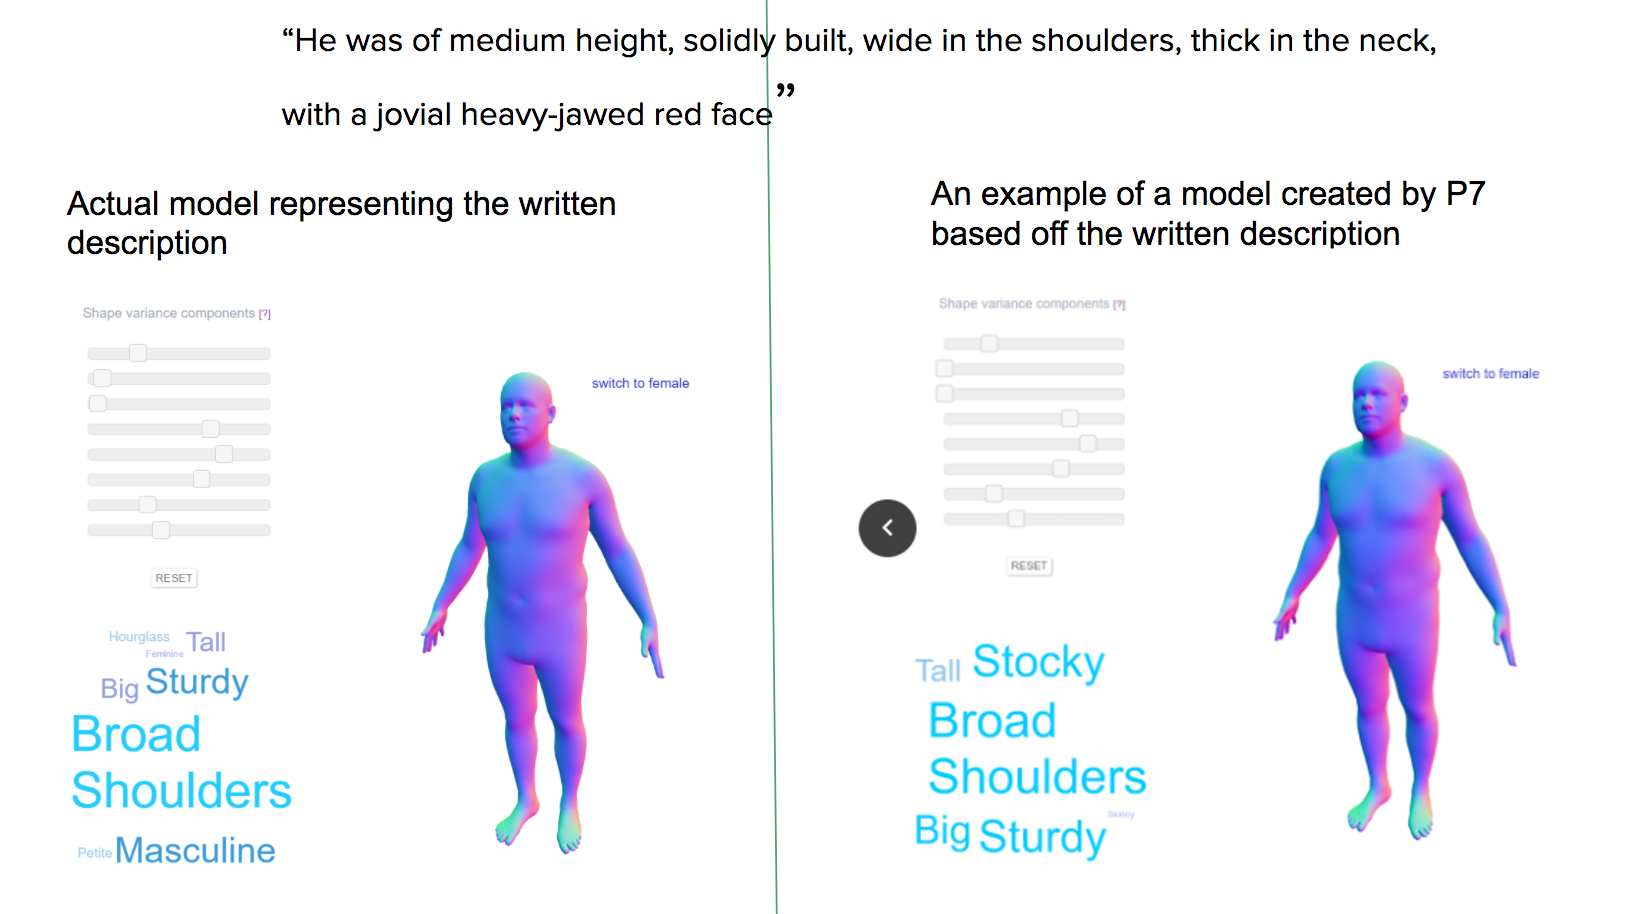
\includegraphics[width=\linewidth]{writtenDescp}
  \caption{An example of a model created both by the algorithm (left) and a participant (right) based on the written description provided at the top.}
	\label{fig:written}
}

%% Uncomment below to disable the manuscript note
%\renewcommand{\manuscriptnotetxt}{}

%% Copyright space is enabled by default as required by guidelines.
%% It is disabled by the 'review' option or via the following command:
% \nocopyrightspace

\vgtcinsertpkg

%%%%%%%%%%%%%%%%%%%%%%%%%%%%%%%%%%%%%%%%%%%%%%%%%%%%%%%%%%%%%%%%
%%%%%%%%%%%%%%%%%%%%%% START OF THE PAPER %%%%%%%%%%%%%%%%%%%%%%
%%%%%%%%%%%%%%%%%%%%%%%%%%%%%%%%%%%%%%%%%%%%%%%%%%%%%%%%%%%%%%%%%

\begin{document}

%% The ``\maketitle'' command must be the first command after the
%% ``\begin{document}'' command. It prepares and prints the title block.

%% the only exception to this rule is the \firstsection command
\firstsection{Introduction}

\maketitle

%% \section{Introduction} %for journal use above \firstsection{..} instead
\noindent Currently, creating 3D visualizations of human bodies is very limited. The only software readily available are expensive 3D body scanners, 
which are restricted to specialized set ups and hard for the average consumer to access or character creators in video games, which are restricted to 
those game worlds. With computers becoming more powerful every year and more capable of producing and rendering 3D models, more specialized 3D modeling
software that is not restricted to experts could prove useful. \newline

\noindent One field which would benefit from the ability to create 3D models is the field
of avatar creation. Avatars are commonly used in 2D applications to provide a visual representation of ones self to the other users of the application.
However, while most hardware allows for the usage of 3D modeling, there is little applications making use of 3D models as avatars. This could be useful
in applications such as teleconferencing where a visual representation of the person talking may allow for a higher level of engagement with the
conversation. Furthermore, 3D avatars have been shown to be successful as mediums for online therapy rooms as they allow for high engagement
and empathy between the caretaker and the participant\cite{Rijn:2015:BJGC}. An important aspect of these avatar-based systems is that they rely
heavily upon identification with the avatar that is created. In order for a person to gain the benefits of empathy and engagement through avatars,
they must see themselves be represented through the avatar\cite{Belisle:2010:PM}. \newline

\noindent Another unexplored medium of creating 3D models is the use of words. When a person describes a certain shape, different words can be used to
create a mental representation of the object the person is describing. Words like "short" or "stocky" may be used to describe a character
like George Costanza from Seinfeld or an actor like Danny Devito. Humans have a generally shared understanding of how these words may be used
to describe a person. By applying the shared understanding of how textual descriptions may be used to describe and create a mental picture of
a body shape, Streuber et al. created Body Talk\cite{Streuber:2016:SIGGRAPH}. Using text-based descriptions to create models may be useful
in the field of criminology when using victim and witness testimonies to try and find a culprit during a case. Text-based descriptions may
also be used when attempting to visualize characters from novels or other text-based mediums. \newline

\noindent Body Talk allows for the creation of 3D models on a website\cite{bodytalk:website} with word descriptor sliders being used to change the 
dimensions 
and shape of the 3D model. However, Streuber et al. did not evaluate the effectiveness of the model's created despite the author's intended goal
of having these new visualizations be used in other applications by users. In our study, our participants attempted to create models using
the Body Talk website that they felt represented themselves. We are interested in whether these visualizations accurately represent themselves
and could be used in avatars in other settings. We also evaluated our participant's ability to create models based purely on a text
description to represent the use case of visualizing a character from a novel or a crime victim report.

\subsection{Background}
\subsubsection{Algorithm}
\noindent Body Talk was developed by a group of researchers at the Max-Planck Institute for Intelligent Systems. The authors originally ran a series
of studies using Amazon Turk to evaluate a series of 17 photographs on how much they corresponded to a set of descriptive words. \
\begin{figure}[!htb]
	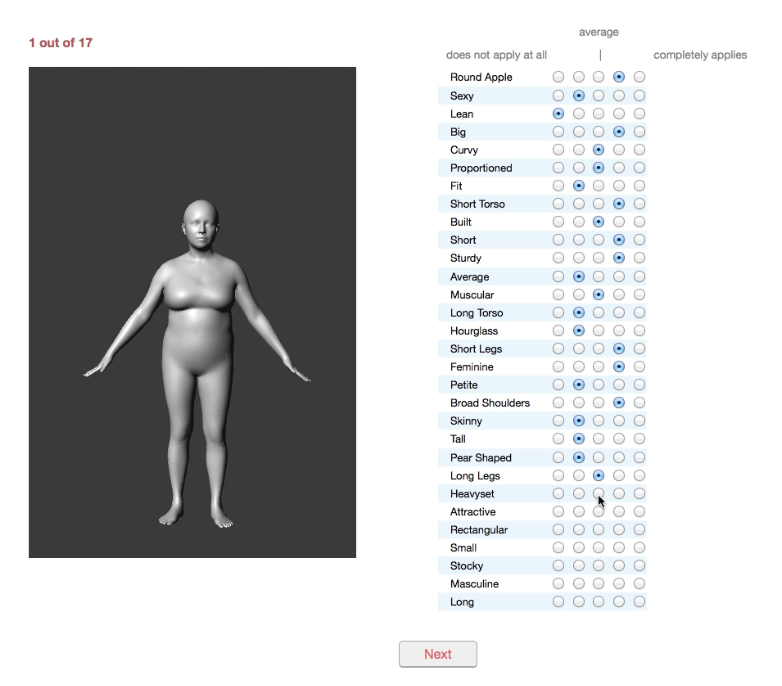
\includegraphics[width=\columnwidth]{survey}
	\caption{Survey on Amazon MTurk}
\end{figure}
Using this crowdsourcing, attribute ratings are generated based off of standard linguistic descriptions of 3D shape. In total, the 
survey was able to gather 15 ratings for each word descriptor over a total of 256 bodies(128 Male, 128 Female). The next major step was 
to generate a linear function that relates the ratings of the words to the 3D model. Additionally some descriptors are correlated 
meaning that words like "skinny" and "petite" should influence each other. The algorithm takes this into account by adjusting these 
particular ratings by their standard deviation, and conditioning for a vector that is used in the 3D model.


\begin{figure}[!htb]
	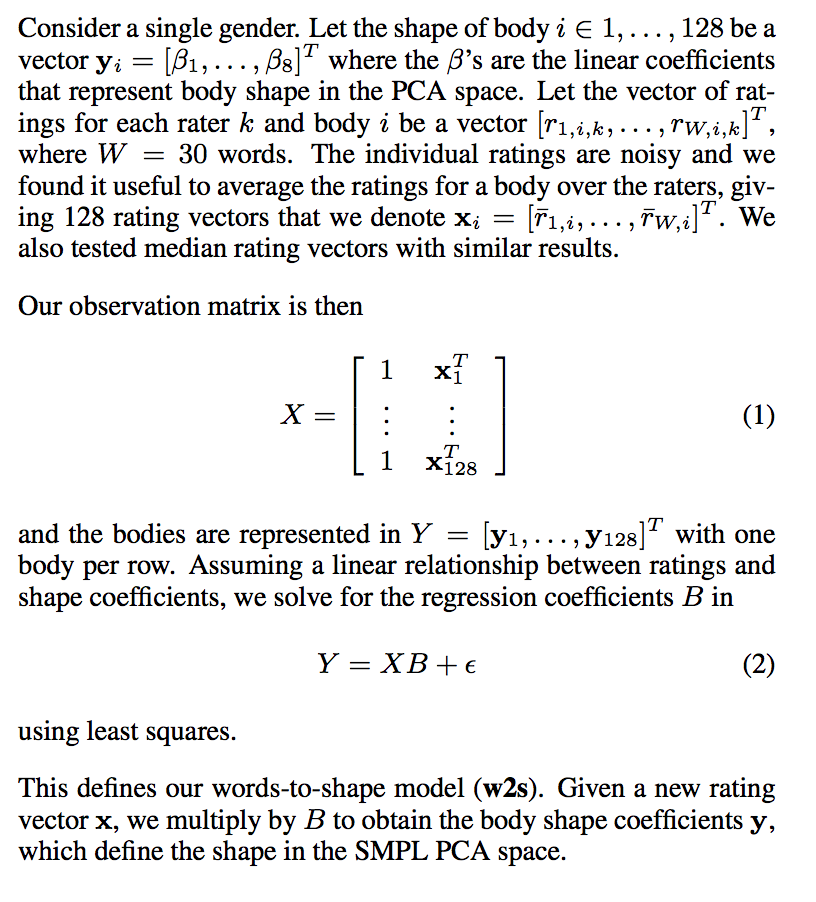
\includegraphics[width=\columnwidth]{algo}
	\caption{Linear function created from dataset}
\end{figure}

\subsubsection{Body Talk Website}
\noindent The website allows for the user to manipulate sliders corresponding to different words that may be used to describe a person. 
\begin{figure} [!htb] 
 \centering
  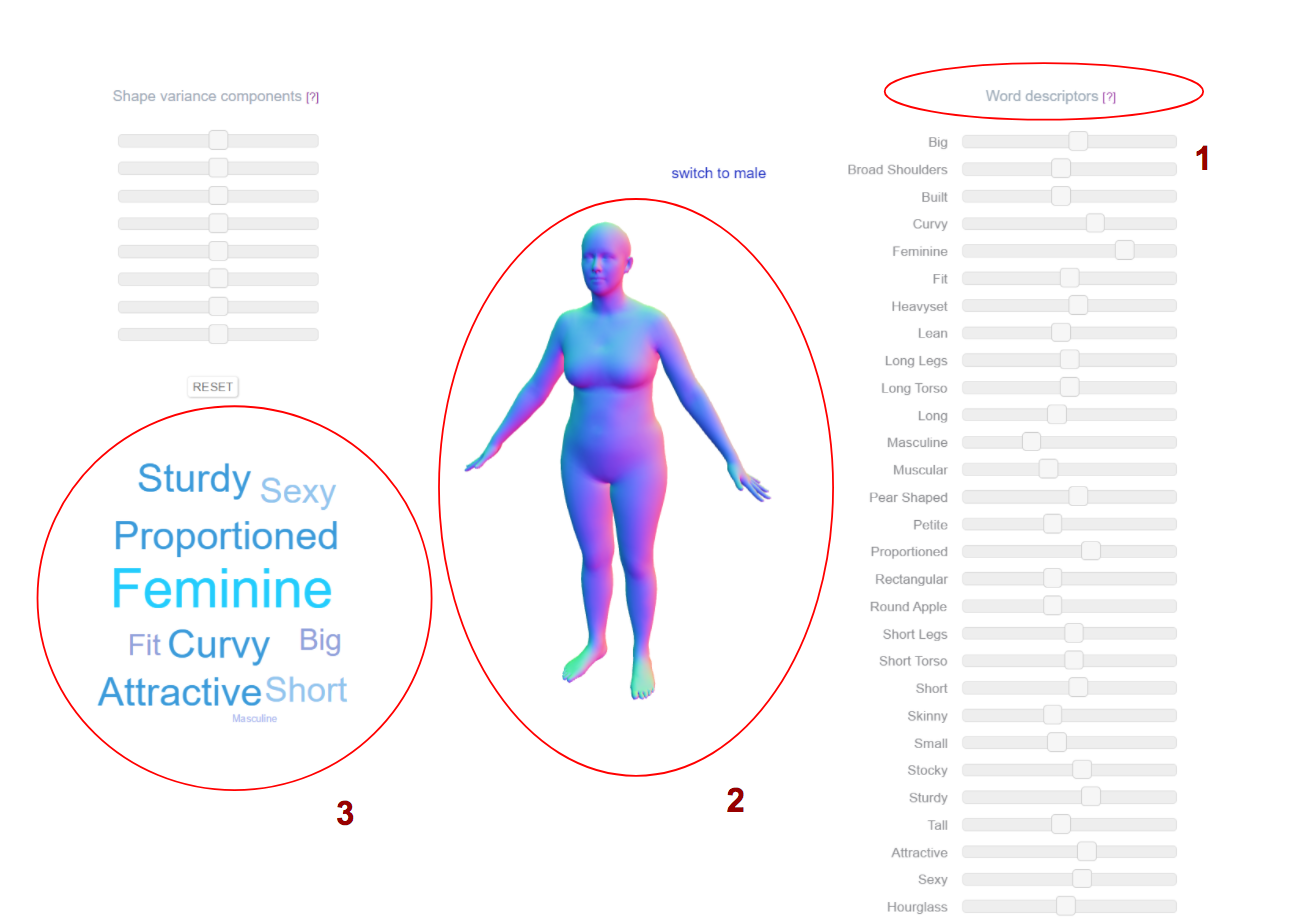
\includegraphics[width=\linewidth]{websiteUI}
  \caption{A screenshot of the Body Talk website. (1) shows the Word Descriptor sliders; (2) shows the model generated by the current configuration of 
  the sliders; (3) shows the outputted word cloud generated based upon the current configuration of sliders}
  \label{fig:websiteUI}
\end{figure}
These 30 words were selected via previous research done by Hill et al.\cite{Hill:15}. Figure \ref{fig:websiteUI} shows what the Body Talk website 
looks like to a user. 
The sliders under Figure \ref{fig:websiteUI}.1 show the various word descriptors. Note that some of these word descriptors are paired, i.e.
if a user slides the "Big" slider to the right, the system will automatically slide sliders such as "Small" to the left or "Heavyset" to the right
to prevent the creation of unrealistic body models. This "enforced word correlation" may be turned off, but, since we were partially
evaluating the effectiveness of enforced word correlation through our creation of models using purely text-based descriptions, we did not inform our
participants of the existence of this slider during the course of the task. After every change in the slider's values, the model shown in Figure 
\ref{fig:websiteUI}.2 is updated. While the model is automatically generated with the change of a slider's value, the word cloud seen in Figure 
\ref{fig:websiteUI}.3 is also updated. These words should match how a person would describe this model's body shape. They can also be used as a way
to validate a textual description provided of a person.


\section{Related Work}
CESAR Dataset
Will add links from last paper...
\section{Methodology}

\section{Results}

\noindent Data was gathered from the user studies to determine whether Body Talk would be viable in other applications. All 7 Oregon State University 
students who took part in these user studies were able to make models they felt accurately depicted their body shape. On a 1 to 5 scale, the average 
student gave their generated model a 4 on how closely the model resembled them. These results show that Body Talk could indeed be useful in generating 
realistic body types from words (students used sliders for each word in the interface). \newline
\begin{figure}[!htb]
	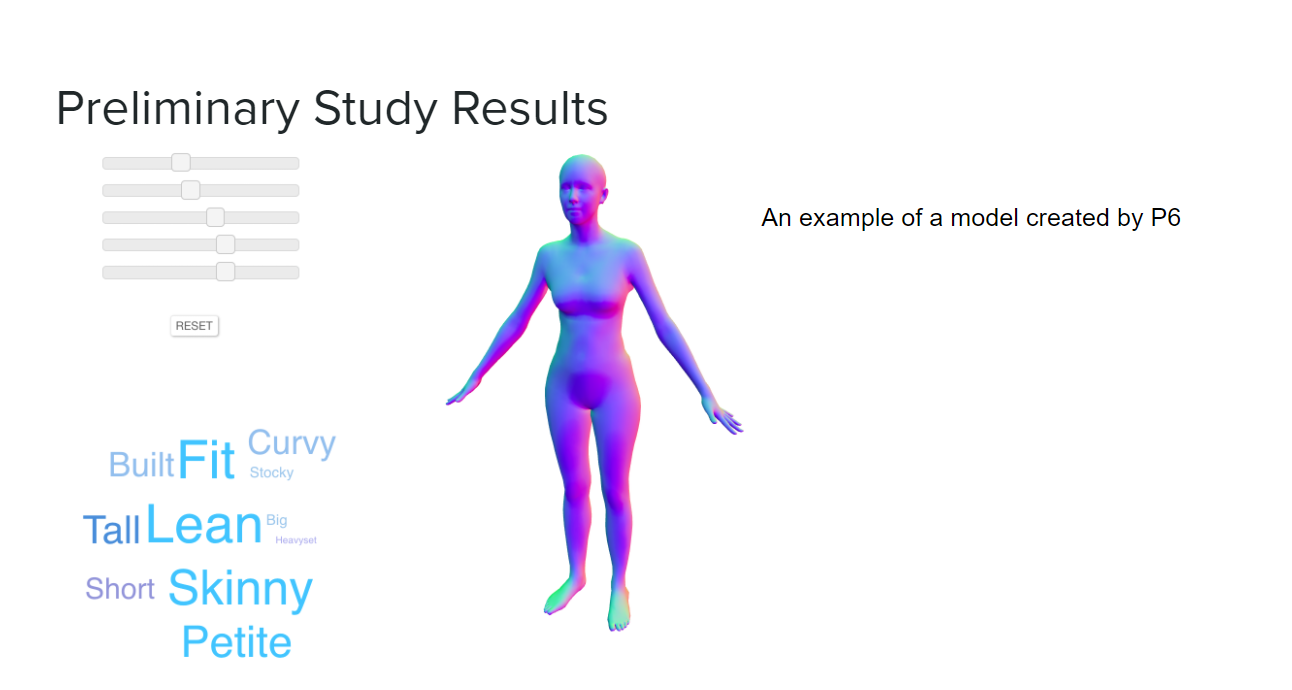
\includegraphics[width=\columnwidth]{user_self_creation.png}
	\caption{This figure shows a model created by a participant. This model is generated during the first part of the study where the participant is asked to create a model of themselves.}
\end{figure}
\noindent However, aside from these impressive stats, the students gave the word descriptions generated from their models a 3.6 out of 5 on whether  they 
believed the words described their body types accurately. This score is okay but not great like the previous score. This is no surprise because Body Talk 
generated around 6 - 16 words for different models. With that many body type descriptions generated, there is bound to by some words that a students just 
wont agree with. Rightfully so, some of the word traits would probably not match their body types at all. Aside from Body Talk generating inaccurate body 
type word descriptions, it also generated very accurate ones as well. This would result in a higher score for this test. But just because a student gives 
a high score, it doesn't mean that it is accurate data. For example, a student may get a "fit" word description generated by Body Talk based off the 
model the student made of themselves. Even if the person really isn't fit, the student may like to see this trait anyways. Because the program gave them 
a positive trait, they will give the test a higher score resulting in inaccurate data. The same thing can happen the other way around. A student may find 
a bad trait that may be true but they don't like, so they give the test a lower score than it should be. All these factors most likely played a factor in 
the user tests which led to a passable average score. Out of the 7 students, 4 of them said they would use their model in other 3D applications. This in no way proves that Body Talk is applicable in other applications. It was a hit or miss in the experiments. However, most students felt confident about the model they created. Though not all the students seemed to think Body Talk is useful, most students generally agreed that its model generation was pretty accurate. \newline

\noindent       

\section{Future Work}

Can include improvements to user studies (ex. set time, more participants, more generated models, more tests) 

\noindent Future work to determine whether Body Talk is useful in other 3D applications is critical. Aside from just getting more data, previous user studies had some flaws that should be fixed. 
\newline \newline
\noindent For example, no set period of time was given for each student to complete the study. This resulted in some students spending way more time on tests than others. In turn, usually the students who spent more time on the tests generated models far more accurate than the ones that spent less time. Future studies will include set time limits to which each participant must complete. 
\newline\newline
\noindent Another limitation of the previous user studies was having no set way to do each test. For example, some students may have done the test face to face. Some may have just gotten an email with all the necessary information to do the tests on their own. Some students may have used a small laptop with a touch screen while others used a computer with a large monitor. All user studies in the future will be done face to face in order to monitor time and the student taking the test. Studies will also include a set computer with a large monitor and working mouse. User using a small screen could not see all the sliders well. They were also having trouble adjusting sliders on a touch screen. This led to frustration which led to worst results which Body Talk is not responsible for. 
\newline\newline
\noindent Aside from these limitations, getting more data and participants would give a more accurate understanding on whether Body Talk is practical in other fields. Future studies will include more students participating in the user studies and students creating more models than just the two.  
  



\subsection{Mezcal Head}

Lorem ipsum dolor sit amet (see \autoref{fig:sample}), consetetur sadipscing elitr, sed diam
nonumy eirmod tempor invidunt ut labore et dolore magna aliquyam erat,
sed diam voluptua. At vero eos et accusam et justo duo dolores et ea
rebum. Stet clita kasd gubergren, no sea takimata sanctus est Lorem
ipsum dolor sit amet. Lorem ipsum dolor sit amet, consetetur
sadipscing elitr, sed diam nonumy eirmod tempor invidunt ut labore et
dolore magna aliquyam erat, sed diam voluptua. At vero eos et accusam
et justo duo dolores et ea rebum. Stet clita kasd gubergren, no sea
takimata sanctus est Lorem ipsum dolor sit amet. 

\subsubsection{Duis Autem}

Lorem ipsum dolor sit amet, consetetur sadipscing elitr, sed diam
nonumy eirmod tempor invidunt ut labore et dolore magna aliquyam erat,
sed diam voluptua. At vero eos et accusam et justo duo dolores et ea
rebum. Stet clita kasd gubergren, no sea takimata sanctus est Lorem
ipsum dolor sit amet. Lorem ipsum dolor sit amet, consetetur
sadipscing elitr, sed diam nonumy eirmod tempor invidunt ut labore et
dolore magna aliquyam erat, sed diam voluptua. At vero eos et accusam
et justo duo dolores et ea rebum. Stet clita kasd gubergren, no sea
takimata sanctus est Lorem ipsum dolor sit amet. Lorem ipsum dolor sit
amet, consetetur sadipscing elitr, sed diam nonumy eirmod tempor
invidunt ut labore et dolore magna aliquyam erat, sed diam
voluptua. At vero eos et accusam et justo duo dolores et ea
rebum. Stet clita kasd gubergren, no sea takimata sanctus est. Lorem
ipsum dolor sit amet.

\begin{figure}[tb]
 \centering % avoid the use of \begin{center}...\end{center} and use \centering instead (more compact)
 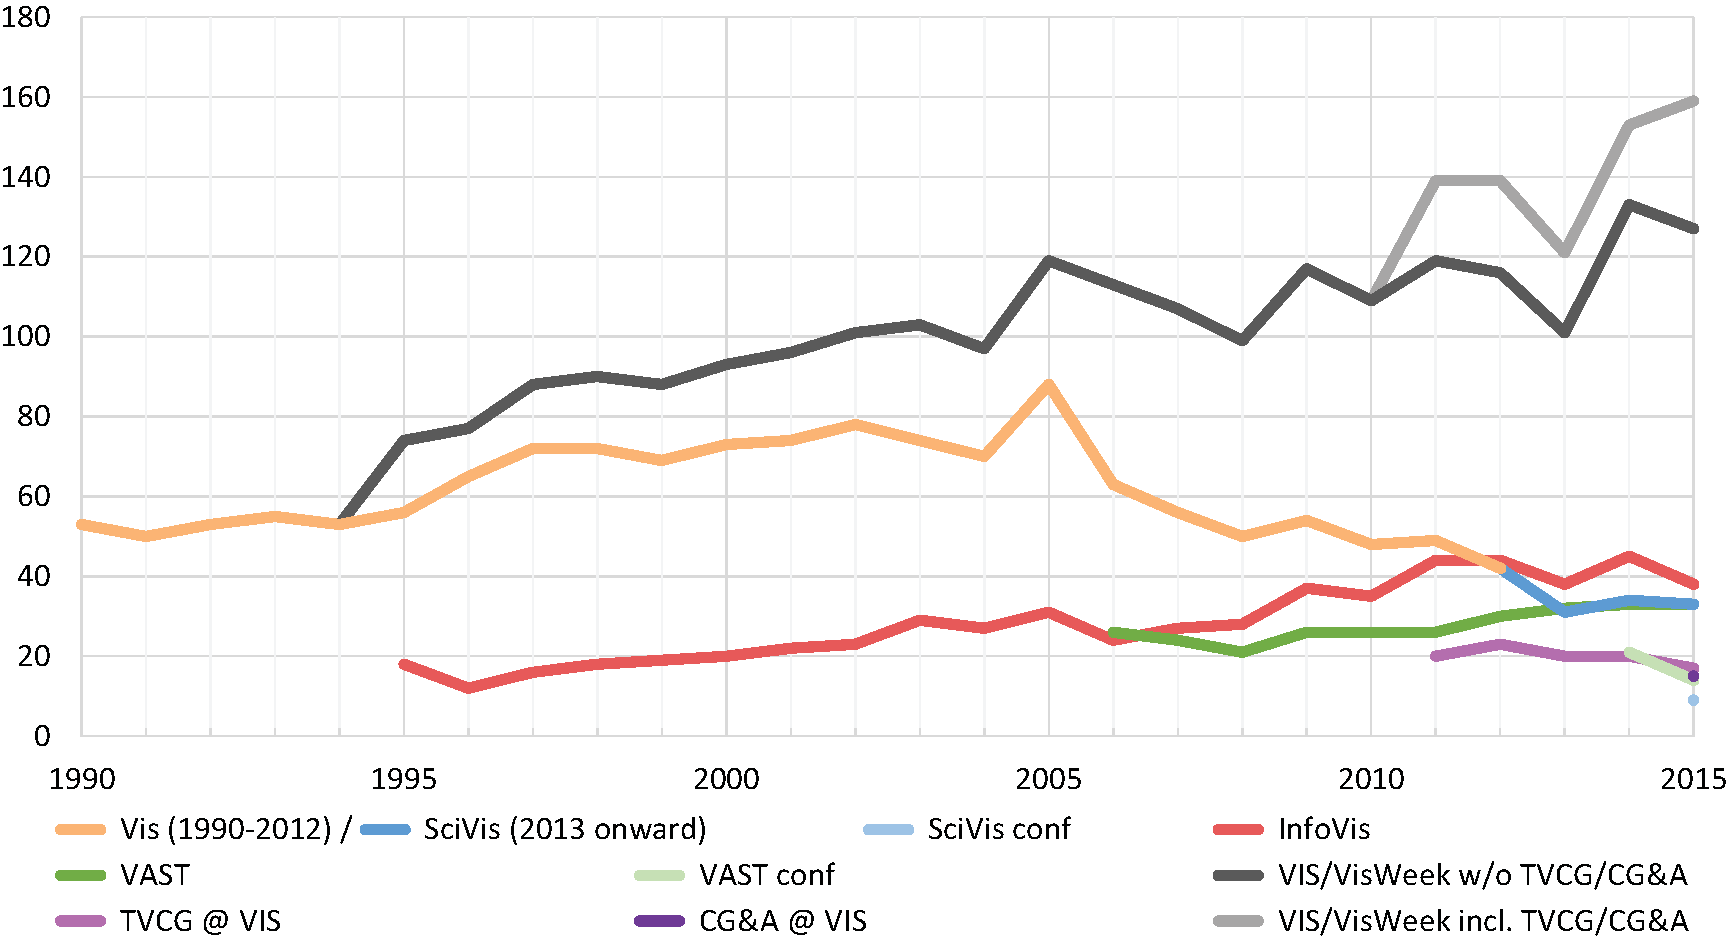
\includegraphics[width=\columnwidth]{paper-count-w-2015-new}
 \caption{A visualization of the data from \autoref{tab:vis_papers}. The image is from \cite{Isenberg:2017:VMC} and is in the public domain.}
 \label{fig:sample}
\end{figure}

\subsubsection{Ejector Seat Reservation}

Duis autem~\cite{Lorensen:1987:MCA}\footnote{The algorithm behind
Marching Cubes \cite{Lorensen:1987:MCA} had already been
described by Wyvill et al. \cite{Wyvill:1986:DSS} a year
earlier.} vel eum iriure dolor in hendrerit
in vulputate velit esse molestie consequat,\footnote{Footnotes
appear at the bottom of the column.} vel illum dolore eu
feugiat nulla facilisis at vero eros et accumsan et iusto odio
dignissim qui blandit praesent luptatum zzril delenit augue duis
dolore te feugait nulla facilisi. Lorem ipsum dolor sit amet,
consectetuer adipiscing elit, sed diam nonummy nibh euismod tincidunt
ut laoreet dolore magna aliquam erat volutpat.


\paragraph{Confirmed Ejector Seat Reservation}

Ut wisi enim ad minim veniam, quis nostrud exerci tation ullamcorper
suscipit lobortis nisl ut aliquip ex ea commodo
consequat~\cite{Nielson:1991:TAD}. Duis autem vel eum iriure dolor in
hendrerit in vulputate velit esse molestie consequat, vel illum dolore
eu feugiat nulla facilisis at vero eros et accumsan et iusto odio
dignissim qui blandit praesent luptatum zzril delenit augue duis
dolore te feugait nulla facilisi.

\paragraph{Rejected Ejector Seat Reservation}

Ut wisi enim ad minim veniam, quis nostrud exerci tation ullamcorper
suscipit lobortis nisl ut aliquip ex ea commodo consequat. Duis autem
vel eum iriure dolor in hendrerit in vulputate velit esse molestie


\section{Conclusion}

Lorem ipsum dolor sit amet, consetetur sadipscing elitr, sed diam
nonumy eirmod tempor invidunt ut labore et dolore magna aliquyam erat,
sed diam voluptua. At vero eos et accusam et justo duo dolores et ea
rebum. Stet clita kasd gubergren, no sea takimata sanctus est Lorem
ipsum dolor sit amet. Lorem ipsum dolor sit amet, consetetur
sadipscing elitr, sed diam nonumy eirmod tempor invidunt ut labore et
dolore magna aliquyam erat, sed diam voluptua. At vero eos et accusam
et justo duo dolores et ea rebum. Stet clita kasd gubergren, no sea
takimata sanctus est Lorem ipsum dolor sit amet. Lorem ipsum dolor sit
amet, consetetur sadipscing elitr, sed diam nonumy eirmod tempor
invidunt ut labore et dolore magna aliquyam erat, sed diam
voluptua. At vero eos et accusam et justo duo dolores et ea
rebum.


%% if specified like this the section will be committed in review mode
\acknowledgments{
The authors wish to thank A, B, C. This work was supported in part by
a grant from XYZ.}

%\bibliographystyle{abbrv}
\bibliographystyle{abbrv-doi}
%\bibliographystyle{abbrv-doi-narrow}
%\bibliographystyle{abbrv-doi-hyperref}
%\bibliographystyle{abbrv-doi-hyperref-narrow}

\bibliography{template}
\end{document}

